% Generated by pysimcount.pffigure -- do not edit; regenerate instead.
% figure: A-tte-by-order -- Suzuki formulas of each order, r from: Commutator bound (2021)
% source: results/pf-thesis/results.json
% metric=cnot gatebase=cz merged
% seed=1 t=n template=simcount synth=pygridsynth
% git_commit=04cd66abb614bdc66fb48e891cef085a299e0ab1 git_dirty=False
% source_sha256=018e0b7603e6fc9f6ee358974f241415a3b93437700847b033937cc1d4250db8
% derived: A-tte-by-order.tex with Lie-Trotter S1 removed by pysimcount.figdrop (Lie-Trotter S1 alone spans 56% of the original y-axis); removed legends: Lie-Trotter S1; source_sha256=c5c6ae47958ce8af4d90edf9771f40fbd48a0926747faea75f6b0198bcc0ceb4
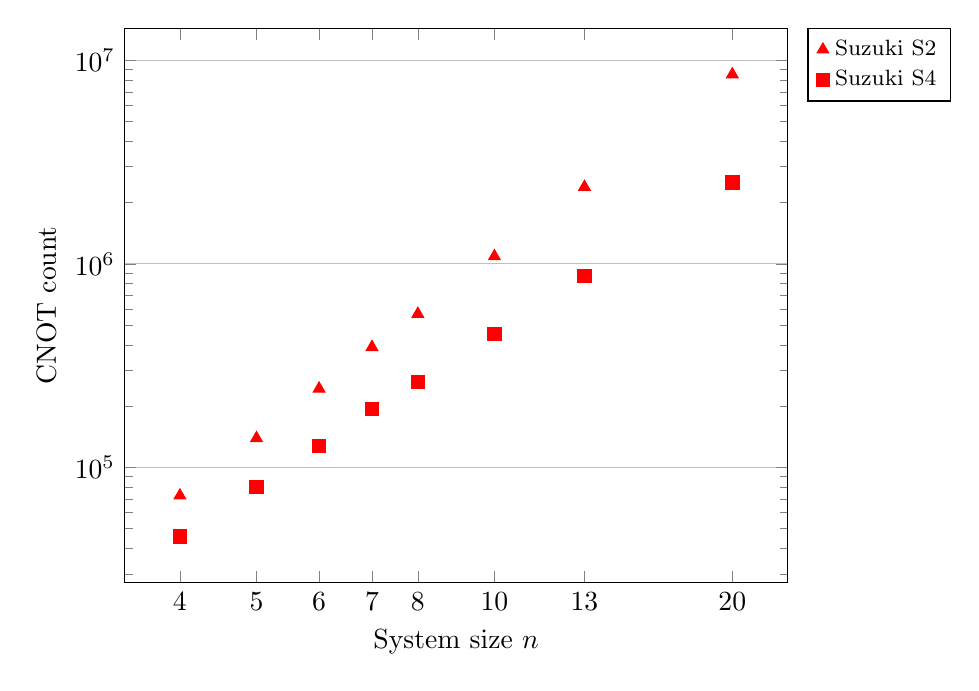
\begin{tikzpicture}
  \begin{loglogaxis}[
    width=10cm,
    xlabel={System size $n$},
    ylabel={CNOT count},
    xtick={4,5,6,7,8,10,13,20},
    xticklabels={4,5,6,7,8,10,13,20},
    ymajorgrids=true,
    legend pos=outer north east,
    legend cell align=left,
    legend style={font=\footnotesize},
  ]
    \addplot[only marks, red, mark=triangle*, mark size=2.4pt, mark options={solid, fill=red}] coordinates {
      (4,72680)
      (5,139050)
      (6,243540)
      (7,389690)
      (8,567040)
      (10,1088000)
      (13,2384070)
      (20,8519400)
    };
    \addlegendentry{Suzuki S2}
    \addplot[only marks, red, mark=square*, mark size=2.4pt, mark options={solid, fill=red}] coordinates {
      (4,45696)
      (5,80010)
      (6,127764)
      (7,193452)
      (8,262080)
      (10,452340)
      (13,872508)
      (20,2509080)
    };
    \addlegendentry{Suzuki S4}
  \end{loglogaxis}
\end{tikzpicture}
